\documentclass[border=0pt,10pt]{standalone}
\usepackage[T1]{fontenc}
\usepackage{lmodern}
\usepackage{pgfplots}
\pgfplotsset{compat=1.17}
\usepgfplotslibrary{groupplots}
\usepackage{xcolor}
\definecolor{oi-blue}{HTML}{0072B2}
\definecolor{oi-vermillion}{HTML}{D55E00}
\definecolor{oi-green}{HTML}{009E73}
\definecolor{oi-purple}{HTML}{CC79A7}
\definecolor{oi-black}{HTML}{000000}
% semantic_sha256: bd2a953e6fdeba82f892112e77e569b479863bd0d1672a21f119ca1f80c333bc
\begin{document}
\begin{minipage}{181.86mm}
\centering
{\bfseries\fontsize{10}{12}\selectfont PP-U-SG | D3 | final\_refit}\\[2mm]
{\fontsize{8}{10}\selectfont planned=42, monitored=42, missing-history=0, status=complete\_history\_coverage}\\[3mm]
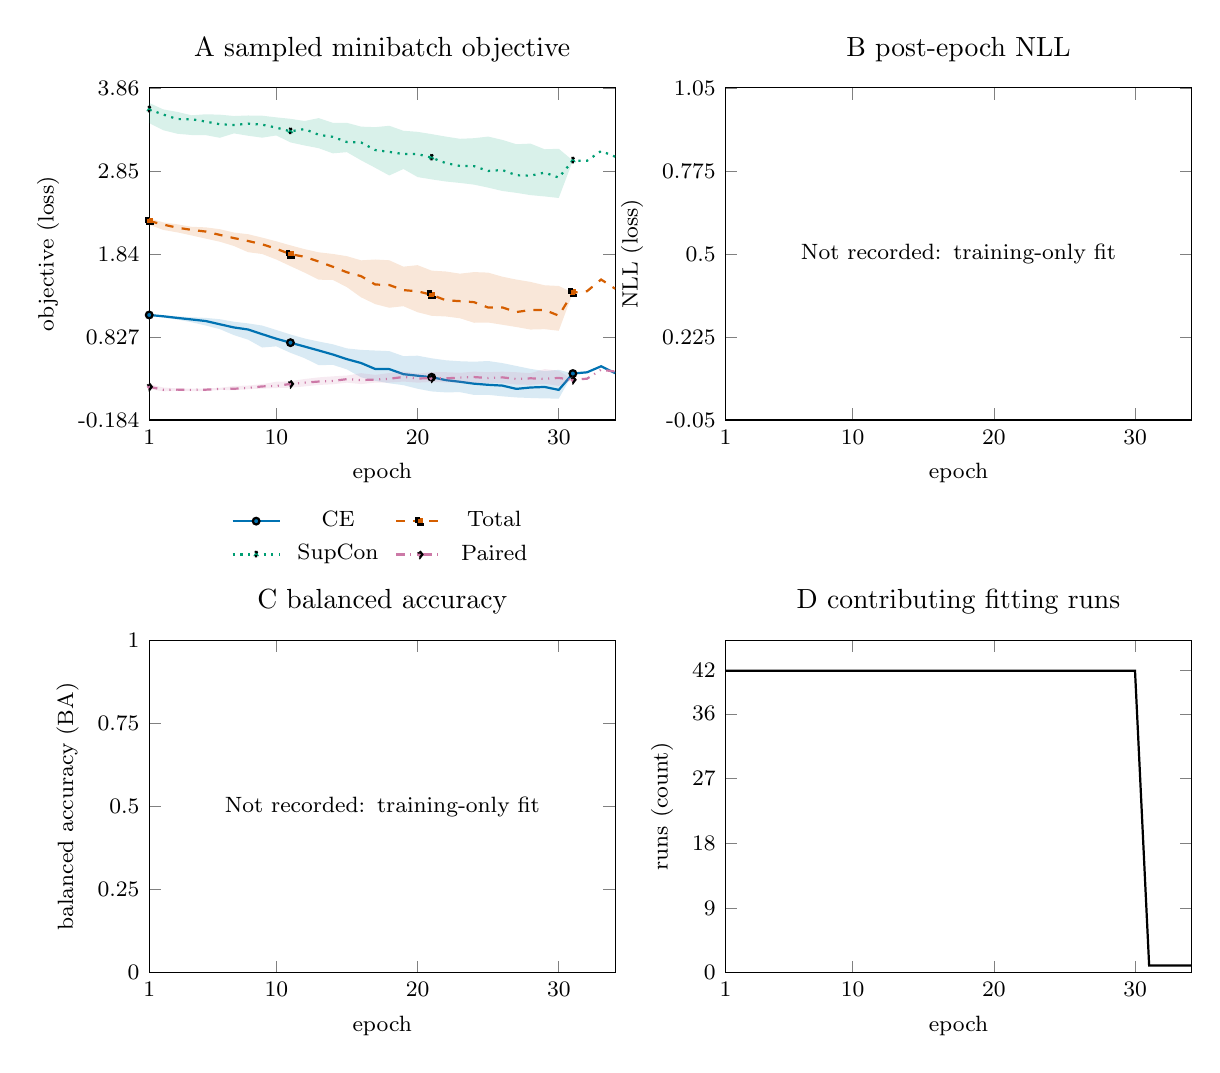
\begin{tikzpicture}
\begin{groupplot}[group style={group size=2 by 2, horizontal sep=14mm, vertical sep=28mm}]
\nextgroupplot[width=75mm, height=58mm, title={A sampled minibatch objective}, xlabel={epoch}, ylabel={objective (loss)}, xmin=1, xmax=34, xtick={1,10,20,30}, ymin=-0.18368585109710694, ymax=3.8574028730392458, ytick={-0.18368585109710694,0.82658632993698133,1.8368585109710696,2.8471306920051576,3.8574028730392458}, yticklabels={-0.184,0.827,1.84,2.85,3.86}, tick label style={font=\fontsize{8}{9}\selectfont, text=black}, label style={font=\fontsize{8}{9}\selectfont, text=black}, title style={font=\fontsize{10}{11}\selectfont, text=black}, legend style={at={(0.5,-0.24)},anchor=north,draw=none,fill=none,font=\fontsize{8}{9}\selectfont,row sep=1pt,column sep=4pt,legend columns=2}]
\addplot[fill=oi-blue,opacity=0.15,draw=none,forget plot] coordinates {(1,1.0872956573963166) (2,1.0620929956436158) (3,1.0383284717798233) (4,1.0062978953123092) (5,0.96610653847455974) (6,0.9221980035305023) (7,0.84909796267747883) (8,0.79424593895673756) (9,0.69860529601573951) (10,0.71255738586187367) (11,0.63407193273305895) (12,0.56898303404450423) (13,0.48340278044342999) (14,0.48791863098740579) (15,0.43220642656087876) (16,0.3361477918922901) (17,0.2943817920982838) (18,0.2630903571844101) (19,0.24062433056533336) (20,0.19685640223324299) (21,0.16424811892211438) (22,0.15281794574111701) (23,0.15562826655805112) (24,0.12207023575901986) (25,0.12321041692048311) (26,0.10508026108145714) (27,0.090983038768172264) (28,0.084397176560014497) (29,0.079186989739537236) (30,0.077110822591930625) (31,0.38217398524284363) (32,0.39695753902196884) (33,0.47045300155878067) (34,0.38599483668804169) (34,0.38599483668804169) (33,0.47045300155878067) (32,0.39695753902196884) (31,0.38217398524284363) (30,0.42684149742126465) (29,0.412002207711339) (28,0.43859193474054337) (27,0.47416046187281607) (26,0.50932526662945743) (25,0.53442201316356652) (24,0.52581521645188334) (23,0.53169115856289861) (22,0.54348512664437298) (21,0.56720574349164965) (20,0.59914223626255991) (19,0.59338211566209798) (18,0.65474412739276877) (17,0.66202673763036723) (16,0.66962627768516536) (15,0.68779683113098145) (14,0.73794976621866226) (13,0.77129140198230739) (12,0.80875143110752101) (11,0.85721332877874368) (10,0.91169377267360685) (9,0.96572748273611064) (8,0.99199894666671751) (7,1.0122048869729041) (6,1.0427245378494263) (5,1.05910624563694) (4,1.066616678237915) (3,1.0782439321279527) (2,1.0902361750602723) (1,1.1036561906337738)};
\addplot[color=oi-blue, mark=*, mark options={draw=black}, mark repeat=10, mark size=1.2pt, solid, line width=0.8pt] coordinates {(1,1.0943706780672073) (2,1.0784210413694382) (3,1.0584486871957779) (4,1.0400125086307526) (5,1.0207914412021637) (6,0.98127557337284088) (7,0.94269928336143494) (8,0.91783010214567184) (9,0.86099128425121307) (10,0.8053123876452446) (11,0.75744400173425674) (12,0.71034926921129227) (13,0.66270057111978531) (14,0.61353451758623123) (15,0.55700898915529251) (16,0.51000469923019409) (17,0.43754704669117928) (18,0.4358842633664608) (19,0.37442302331328392) (20,0.35545104742050171) (21,0.33709623664617538) (22,0.30224540457129478) (23,0.28184125572443008) (24,0.25864582322537899) (25,0.24479850754141808) (26,0.23526733834296465) (27,0.19536222144961357) (28,0.21215800847858191) (29,0.21864703577011824) (30,0.18309915252029896) (31,0.38217398524284363) (32,0.39695753902196884) (33,0.47045300155878067) (34,0.38599483668804169)};
\addlegendentry{CE}
\addplot[fill=oi-vermillion,opacity=0.15,draw=none,forget plot] coordinates {(1,2.1914769828319551) (2,2.1290595054626467) (3,2.0990591168403627) (4,2.062182602286339) (5,2.0237389415502549) (6,1.9857838600873947) (7,1.9335523515939712) (8,1.8583877563476563) (9,1.8360894650220871) (10,1.7691795915365218) (11,1.6887652218341827) (12,1.6099044173955919) (13,1.5237461447715759) (14,1.5207983613014222) (15,1.4323998868465424) (16,1.3094675153493882) (17,1.2265548825263977) (18,1.1823507100343704) (19,1.2012625068426133) (20,1.1280856341123582) (21,1.0843863815069199) (22,1.0764140099287034) (23,1.0545855477452277) (24,0.99976485818624494) (25,1.0029400378465652) (26,0.97562605142593384) (27,0.94791008681058886) (28,0.91714610755443571) (29,0.92187740206718449) (30,0.9023153021931648) (31,1.3659708499908447) (32,1.3836656212806702) (33,1.5257362425327301) (34,1.4136682152748108) (34,1.4136682152748108) (33,1.5257362425327301) (32,1.3836656212806702) (31,1.3659708499908447) (30,1.4473745793104171) (29,1.4559691548347473) (28,1.4966495096683503) (27,1.525269976258278) (26,1.5603954493999481) (25,1.6098094552755355) (24,1.6162991791963577) (23,1.5971770018339158) (22,1.6236446887254714) (21,1.6338798582553864) (20,1.7005879342555998) (19,1.6825007259845735) (18,1.7597180485725401) (17,1.7694856464862823) (16,1.7593897998332977) (15,1.8097301393747329) (14,1.8370398133993149) (13,1.8569958537817002) (12,1.895441821217537) (11,1.9415912330150604) (10,1.9907105684280395) (9,2.0355906307697298) (8,2.0771839439868929) (7,2.0972831010818482) (6,2.1378900706768036) (5,2.1603970766067504) (4,2.1673964858055115) (3,2.1973035633563995) (2,2.220396715402603) (1,2.2704340219497681)};
\addplot[color=oi-vermillion, mark=square*, mark options={draw=black}, mark repeat=10, mark size=1.2pt, dashed, line width=0.8pt] coordinates {(1,2.237817108631134) (2,2.1936523914337158) (3,2.1563486754894257) (4,2.1298113465309143) (5,2.1093825399875641) (6,2.0687651932239532) (7,2.0299420654773712) (8,1.9943671822547913) (9,1.9546187371015549) (10,1.8996612131595612) (11,1.8343821167945862) (12,1.8025776892900467) (13,1.7444164603948593) (14,1.6811579912900925) (15,1.6138227730989456) (16,1.5668244212865829) (17,1.4653647243976593) (18,1.4585933983325958) (19,1.3970645070075989) (20,1.3826794475317001) (21,1.339609295129776) (22,1.2730823159217834) (23,1.2630458325147629) (24,1.2502801865339279) (25,1.1850063651800156) (26,1.1865945681929588) (27,1.1303168162703514) (28,1.1547771543264389) (29,1.1554673165082932) (30,1.0859739705920219) (31,1.3659708499908447) (32,1.3836656212806702) (33,1.5257362425327301) (34,1.4136682152748108)};
\addlegendentry{Total}
\addplot[fill=oi-green,opacity=0.15,draw=none,forget plot] coordinates {(1,3.4287158370018007) (2,3.3419095098972322) (3,3.2990590512752531) (4,3.2839499652385711) (5,3.2824531078338621) (6,3.2501666843891144) (7,3.3036179840564728) (8,3.275175005197525) (9,3.2516017794609069) (10,3.2785712361335753) (11,3.1938796758651735) (12,3.156584006547928) (13,3.1236374020576476) (14,3.0611038506031036) (15,3.0751506090164185) (16,2.976275271177292) (17,2.8851223111152651) (18,2.7915707349777223) (19,2.8704351782798767) (20,2.7723767042160032) (21,2.7439880788326265) (22,2.7183590531349182) (23,2.7010366916656494) (24,2.6802903890609739) (25,2.6439474403858183) (26,2.6033071815967559) (27,2.5803718030452729) (28,2.5525675356388091) (29,2.5366727411746979) (30,2.5179706931114199) (31,2.9735307693481445) (32,2.9697186946868896) (33,3.0891954302787781) (34,3.01985102891922) (34,3.01985102891922) (33,3.0891954302787781) (32,2.9697186946868896) (31,2.9735307693481445) (30,3.1162997841835023) (29,3.1103442013263702) (28,3.1792548298835754) (27,3.1717770159244538) (26,3.2248417019844053) (25,3.2648252308368684) (24,3.2451130807399751) (23,3.2379563570022585) (22,3.2647620677947997) (21,3.2945919036865234) (20,3.3226542890071871) (19,3.3355539858341219) (18,3.3961757481098176) (17,3.3794888734817503) (16,3.385754293203354) (15,3.4321313560009004) (14,3.4324018001556396) (13,3.4896694242954256) (12,3.4541498839855196) (11,3.4810284614562987) (10,3.49848815202713) (9,3.5189440488815307) (8,3.5214478611946105) (7,3.5149631023406984) (6,3.5313734889030455) (5,3.5361375689506529) (4,3.5239889502525328) (3,3.5646982312202455) (2,3.5955162525177) (1,3.6737170219421387)};
\addplot[color=oi-green, mark=triangle*, mark options={draw=black}, mark repeat=10, mark size=1.2pt, dotted, line width=0.8pt] coordinates {(1,3.5942781269550323) (2,3.532427042722702) (3,3.4775235950946808) (4,3.4764325022697449) (5,3.4474954903125763) (6,3.4145798981189728) (7,3.405526727437973) (8,3.4226312041282654) (9,3.4098511934280396) (10,3.3738081157207489) (11,3.3285857141017914) (12,3.3561800718307495) (13,3.2866900861263275) (14,3.2616027593612671) (15,3.198509156703949) (16,3.1931225955486298) (17,3.1010328531265259) (18,3.0784106254577637) (19,3.0520318150520325) (20,3.052519828081131) (21,3.0076069235801697) (22,2.9420516788959503) (23,2.9076801240444183) (24,2.905201643705368) (25,2.8467629849910736) (26,2.858010858297348) (27,2.7940526306629181) (28,2.788534015417099) (29,2.8268364369869232) (30,2.7659574449062347) (31,2.9735307693481445) (32,2.9697186946868896) (33,3.0891954302787781) (34,3.01985102891922)};
\addlegendentry{SupCon}
\addplot[fill=oi-purple,opacity=0.15,draw=none,forget plot] coordinates {(1,0.19262175597250461) (2,0.16554624028503895) (3,0.17087012529373169) (4,0.16732233725488185) (5,0.16930656768381597) (6,0.18286089450120926) (7,0.18014583215117455) (8,0.19124187417328359) (9,0.19800271466374397) (10,0.20575071834027767) (11,0.21004145815968514) (12,0.2252815306186676) (13,0.24323311299085618) (14,0.25137326903641222) (15,0.27115354984998702) (16,0.25330322645604608) (17,0.27146547958254813) (18,0.27232703417539594) (19,0.28457859195768831) (20,0.27110241577029226) (21,0.2791717626154423) (22,0.27505234517157079) (23,0.27010738588869571) (24,0.27000142820179462) (25,0.26886368133127692) (26,0.26582722812891008) (27,0.24806098788976669) (28,0.24448113664984703) (29,0.2580275248736143) (30,0.23161390386521816) (31,0.30579210072755814) (32,0.31930799037218094) (33,0.42841517180204391) (34,0.40572671592235565) (34,0.40572671592235565) (33,0.42841517180204391) (32,0.31930799037218094) (31,0.30579210072755814) (30,0.4154704198241233) (29,0.43643797636032106) (28,0.38652631491422651) (27,0.39788851141929626) (26,0.40460477396845818) (25,0.39851492643356323) (24,0.40489913076162337) (23,0.39130768477916716) (22,0.3981725197285414) (21,0.39998697042465209) (20,0.38121721968054773) (19,0.40643565803766252) (18,0.38822178766131399) (17,0.36562688276171684) (16,0.38659479692578314) (15,0.35765823051333429) (14,0.34803629145026205) (13,0.33541764840483662) (12,0.31523434184491633) (11,0.28785096704959867) (10,0.28205800391733649) (9,0.25275667719542982) (8,0.23594225756824017) (7,0.23006588295102118) (6,0.20834267511963844) (5,0.19984780848026276) (4,0.19846567697823048) (3,0.2009610015898943) (2,0.21243688389658927) (1,0.25229796245694158)};
\addplot[color=oi-purple, mark=diamond*, mark options={draw=black}, mark repeat=10, mark size=1.2pt, dash dot dot, line width=0.8pt] coordinates {(1,0.22094338946044445) (2,0.18435156345367432) (3,0.186176847666502) (4,0.18300007842481136) (5,0.18563975393772125) (6,0.19474598579108715) (7,0.19659867137670517) (8,0.20721953362226486) (9,0.22523143887519836) (10,0.23103596083819866) (11,0.25553037039935589) (12,0.27132092975080013) (13,0.28465953283011913) (14,0.29270199127495289) (15,0.31378505006432533) (16,0.30259810760617256) (17,0.30846997536718845) (18,0.31838347390294075) (19,0.34012288972735405) (20,0.32203497551381588) (21,0.32525202259421349) (22,0.32332265004515648) (23,0.33215339295566082) (24,0.33900533244013786) (25,0.32755952887237072) (26,0.33564559929072857) (27,0.31537917628884315) (28,0.32387272641062737) (29,0.3183076586574316) (30,0.32839754410088062) (31,0.30579210072755814) (32,0.31930799037218094) (33,0.42841517180204391) (34,0.40572671592235565)};
\addlegendentry{Paired}
\nextgroupplot[width=75mm, height=58mm, title={B post-epoch NLL}, xlabel={epoch}, ylabel={NLL (loss)}, xmin=1, xmax=34, xtick={1,10,20,30}, ymin=-0.050000000000000003, ymax=1.05, ytick={-0.050000000000000003,0.22500000000000003,0.5,0.77500000000000002,1.05}, yticklabels={-0.05,0.225,0.5,0.775,1.05}, tick label style={font=\fontsize{8}{9}\selectfont, text=black}, label style={font=\fontsize{8}{9}\selectfont, text=black}, title style={font=\fontsize{10}{11}\selectfont, text=black}]
\node[align=center, text width=55mm, font=\fontsize{8}{9}\selectfont] at (axis cs:17.5,0.5) {Not recorded: training-only fit};
\nextgroupplot[width=75mm, height=58mm, title={C balanced accuracy}, xlabel={epoch}, ylabel={balanced accuracy (BA)}, xmin=1, xmax=34, xtick={1,10,20,30}, ymin=0, ymax=1, ytick={0,0.25,0.5,0.75,1}, yticklabels={0,0.25,0.5,0.75,1}, tick label style={font=\fontsize{8}{9}\selectfont, text=black}, label style={font=\fontsize{8}{9}\selectfont, text=black}, title style={font=\fontsize{10}{11}\selectfont, text=black}]
\node[align=center, text width=55mm, font=\fontsize{8}{9}\selectfont] at (axis cs:17.5,0.5) {Not recorded: training-only fit};
\nextgroupplot[width=75mm, height=58mm, title={D contributing fitting runs}, xlabel={epoch}, ylabel={runs (count)}, xmin=1, xmax=34, xtick={1,10,20,30}, ymin=0, ymax=46.200000000000003, ytick={0,9,18,27,36,42}, yticklabels={0,9,18,27,36,42}, tick label style={font=\fontsize{8}{9}\selectfont, text=black}, label style={font=\fontsize{8}{9}\selectfont, text=black}, title style={font=\fontsize{10}{11}\selectfont, text=black}]
\addplot[color=oi-black, solid, line width=0.8pt] coordinates {(1,42) (2,42) (3,42) (4,42) (5,42) (6,42) (7,42) (8,42) (9,42) (10,42) (11,42) (12,42) (13,42) (14,42) (15,42) (16,42) (17,42) (18,42) (19,42) (20,42) (21,42) (22,42) (23,42) (24,42) (25,42) (26,42) (27,42) (28,42) (29,42) (30,42) (31,1) (32,1) (33,1) (34,1)};
\end{groupplot}
\end{tikzpicture}
\par\vspace{6mm}
\begin{minipage}{175mm}
{\fontsize{8}{10}\selectfont RQ-S01 / Scope E: descriptive training diagnostics. 400-1800 cm-1 inputs: SG uses impulse replacement and Savitzky-Golay smoothing; arPLS uses impulse replacement and baseline correction; both finish with [0,1] min-max scaling. CE = chemical cross-entropy; SupCon = supervised contrastive; Paired = paired consistency; NLL = negative log-likelihood; BA = balanced accuracy. Authenticated complete monitor histories aggregated across unique fitting jobs into descriptive policy/recipe/stage curves. Curves summarize per-epoch minibatch-weighted training chemical cross-entropy and the composite total optimization objective; these sampled minibatch objectives differ from post-epoch evaluation negative log-likelihood. Auxiliary supcon/paired loss components are recipe-specific and are not directly comparable to the total objective across recipes. Validation metrics are recorded for source\_fit runs only and never substitute for a held-out test set; calibration\_model\_fit and final\_refit rows carry training-only diagnostics. Source\_fit optimization uses a 30-epoch minimum stopping threshold and a 200-epoch maximum; refit stages reuse the caller-selected duration. Curves are fitting-run-weighted descriptive summaries over correlated runs (seeds/splits). Lines show medians; 10th/90th percentiles describe variation among saved fitting runs, not confidence intervals. Only runs that reached each epoch contribute; early stopping changes the composition, and stopped runs are not carried forward. Fitting jobs are not independent chemical samples: the dataset has 598 spectra from 69 physical samples and 10 instruments. Coverage is limited to saved SG/arPLS monitor histories; historical MIN losses are not pooled or invented. A missing history is not a zero loss or proof of a failed model. These curves do not support hypothesis tests, superiority claims, model selection, or new uncertainty inference. P08 learned-method performance is reported elsewhere.}
\end{minipage}
\end{minipage}
\end{document}